\chapter{General aspects of using \HS}

\section{Starting up \HS}\label{sec:using_startingUpHS}
The \HS main \ac{VI} (HelioScan_3.vi) cannot be started directly from within the Windows Explorer, but rather needs to be started from within \HS's \LV project browser. 
\begin{enumerate}
	\item If you have multiple \LV versions installed on your set-up computer, start \LV 2010 SP1 and close all other running \LV versions if possible. 
	\item Double-click on the \HS project file (helioscan.lvproj) in the \HS base directory. The \LV project browser window will open, showing you a tree view of project items. Note that the project browser will open in the most recently started \LV version. For \HS to run properly, this needs to be \LV 2010 SP1. If you require running another \LV version simultaneously for some reason, open the \HS project file directly from within \LV 2010 SP1 in order to prevent that it is opening in the wrong \LV version. 
	\item Within the project browser, open the \HS main \ac{VI} by double-clicking on the item Helioscan_3.vi.
	\item Start the \HS main \ac{VI} via the \ac{VI} start button. If it is the first time you are starting up a newly installed \HS version, the start-up process might last several minutes because \LV compiles all \HS files being loaded. Once compiled, starting up \HS typically requires between half a minute and a full minute to load its initial combination of components. During the start-up process, a progress bar indicates the progressive loading of components. Loading is finished and \HS ready for use, when the progress bar has completed and switched its colour from orange to green. 
\end{enumerate}

\section{Shutting down \HS}\label{sec:using_shuttingDownHS}
There are several ways to shut down \HS. Here, they are listed with increasing harshness. We recommend to start with the softest method and work your way down the list in case you are not successful. Due to the complex nature of a running \HS application and its dependency on other software and hardware resources this might sometimes be necessary.
\begin{itemize}
	\item The recommended way to terminate the \HS main \ac{VI} is via the \HS exit button. This will properly terminate all components and release all resources including allocated memory and hardware resources, as indicated by the progress bar. The main \ac{VI} will stay open so you can re-start it if needed. In case the main \ac{VI} keeps hanging during shut-down, proceed with the next harsher method to shut down.
	\item Terminate the \HS main \ac{VI} by clicking its \ac{VI} stop button. This will not execute the shut-down procedures of the individual components, but stop the main \ac{VI} immediately. It will still stay open so you can re-start if needed. If the main \ac{VI} does not react when you press the \ac{VI} stop button, proceed with the next harsher method.
	\item Terminate \LV including \HS by killing the \LV process in the Windows Task Manager. This is to fastest method to shut-down \HS. If you want to restart, you need to proceed as outlined in \prettyref{sec:using_startingUpHS}.
\end{itemize}

\section{\ac{GUI} of the \HS main \ac{VI}}\label{sec:using_mainVIGUI}

%\begin{figure}[h!]
%	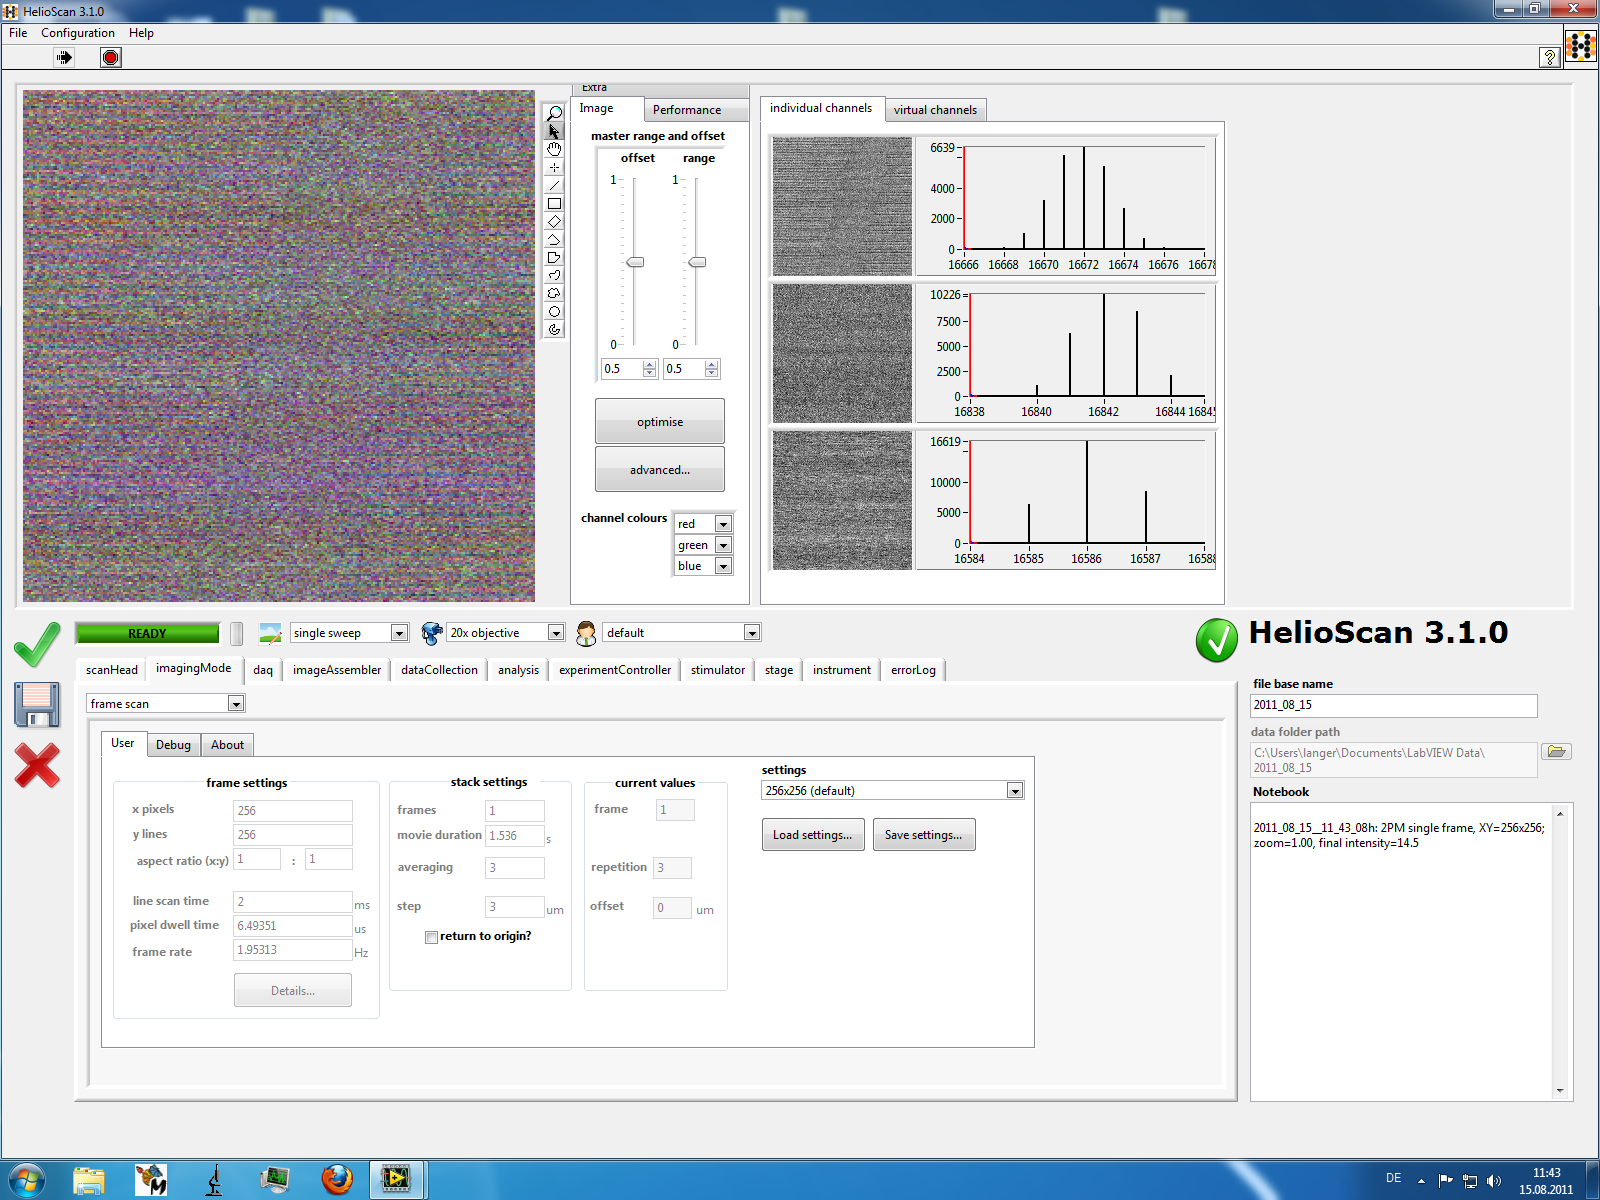
\includegraphics[width=156mm]{figures/using/mainVIGUI/fig.png}
%	\caption {\ac{GUI} of the \HS 3 main \ac{VI}}
%	\label{fig:using_gui}
%\end{figure}

You need to be familiar with the following user interface items of the \HS main \ac{VI} and their respective terms:
\begin{itemize}
	\item \textit{\ac{TLC} tabs:} Each \ac{TLC} owns a dedicated tab into which the respective \ac{TLC}'s \acp{GUI} is loaded at run-time. An exception is the \ac{GUI} of the Display \ac{TLC}, which is not loaded into a \ac{TLC} tab, but owns its own area in the upper half of the main \ac{VI}'s \ac{GUI}. 
	\item \textit{Progress bar:} A multi-colour progress bar indicates the progressive loading and unloading of \acp{TLC} and the readiness of the main \ac{VI}. If all \acp{TLC} are loaded and initialised, the progress bar is at \SI{100}{\percent} and indicates via its green colour that \HS is ready for imaging. If any of the \acp{TLC} is missing, the colour is orange, thus signalling that \HS is not ready for imaging yet. 
	\item \textit{User selector}: This drop-down menu allows choosing between different configuration sets. Basically, each user can have its own set of configuration files stored in subdirectories of the \HS configuration folder (see \prettyref{sec:configuration_preparingSteps}). The names of these subfolders are listed in the drop-down menu and are available for selection. By default, the configuration set contained in the folder "default" is selected.
	\item \textit{Objective selector}: This drop-down menu allows selecting an objective. Use the main configuration dialog of \HS to configure which objectives are available for selection. There, you can also configure the default value of the objective selector. For two reasons, we recommend that you always select the objective that you have effectively in use for your measurement.  First, the objective properties (most importantly, it's magnification factor) are usually stored in the meta-information section of image files generated by \HS (at least of you use a DataCollection \ac{TLC}. Second, the magnification factor of the selected objective is needed for the calculation of the scale bar that can be displayed as an overlay on the image display. 
	\item \textit{ExperimentController selector:} This drop-down menu lists all the ExperimentController configurations added in the \HS main configuration dialog. It allows selecting the ExperimentController instance to be used when imaging in \textit{experiment mode} (see \prettyref{sec:using_runModes}).
	\item \textit{ImagingMode selector:} This drop-down menu lists all ImagingMode configurations added in the \HS main configuration dialog. It allows selecting the ImagingMode instance to be used for imaging. When imaging in \textit{experiment mode} (see \prettyref{sec:using_runModes}), it is important to be aware that certain ExperimentControllers can be configured to automatically choose different ImagingModes or ImagingMode configurations in automated imaging sequences. Other ExperimentControllers always use the ImagingMode that you have previously selected using the ImagingMode selector. When imaging in \textit{single-sweep mode}, \HS always uses the ImagingMode configuration that you specified via the ImagingMode selector.
	\item \textit{Start/stop buttons:} \HS offers three different buttons to start and stop image acquisition. Each button is responsible for a different run mode  (see \prettyref{sec:using_runModes}). From top to bottom, these are the start/stop button for \textit{focus mode}, \textit{single sweep mode} and \textit{experiment mode}. 
	\item \textit{Save button:} Use this button to actively trigger saving of the data you have acquired. In \textit{single-sweep mode}, data acquired during the last sweep will be saved. In \textit{experiment mode}, either data of the last sweep or of the whole sweep series will be saved (depending on the DataCollection \ac{TLC} you are using). Note that certain DataCollection \acp{TLC} give you the option to enable auto-saving, such that each sweep is automatically saved and you do not need to invoke the save button.
	\item \textit{Version indicator:} This indicator displays you are current version of \HS (note that the indicator is dynamically updated during the start-up process, so do not rely on its content before the progress bar is in status \textit{ready}. The indicator also shows (via an orange exclamation mark) when a more recent \HS version is available for download.
	\item \textit{Notebook:} The notebook logs image acquisition details during a measurement session. Notebook log files are automatically and incrementally saved whenever the notebook content changes. This means that for a single imaging session, you typically end up with a large number of notebook files. Since log files names contain a time stamp, you can sort them according to name in Windows Explorer and easily find the most recent version. When you accidentally made an unwanted change to the notebook, you can go back to earlier versions to recover the original information. When saving data to disk, \HS typically adds the name of the save together with some more acquisition details. You are free to manually enter further information anywhere in the already existing notebook content.
	\item \textit{Exit button:} This button  should be used to shut down \HS at the end of a imaging session (see \prettyref{sec:using_shuttingDownHS}).
\end{itemize}

\section{Run modes}\label{sec:using_runModes}
\HS performs image acquisition in one of three run-modes. You as the user decides which run mode is to be used by pressing the corresponding start button (see \prettyref{sec:using_mainVIGUI}).
\begin{itemize}
	\item \textit{Focus mode:} In this run mode, image acquisition continues until stopped again by the user via the corresponding start/stop button. Use this run mode to find you region of interest in the specimen and to adjust imaging conditions (such as illumination power).
	\item \textit{Single-sweep mode:} In this run mode, image acquisition continues for the number of frames or duration specified in the currently active ImagingMode. Acquired images are temporarily stored until you press the safe button or start a new sweep.
	\item \textit{Experiment mode:} In this run mode, control over image acquisition is handed over to the currently active ExperimentController \ac{TLC}. The ExperimentController is typically used to perform a series of sweeps in a row. Depending on the ExperimentController used, sweep acquisition may for expample be started in regular time intervals or upon hardware triggers. 
\end{itemize}